\chapter{Velocity and Angle estimation}
To give a better position estimate which can be fed to the controller as well, the different data collected from the sensors mounted are put through a Kalman filter. This filter takes the different measurements as inputs, and uses these to give a better estimate of the position, rather than the quite noisy measurements taken using just the raw \ac{GPS} data. 

To develop such a filter, the model of the ship is to be computed, as well as a mapping of the different inputs and outputs to the system. The model of the forward and sidewards case (surge and sway) are the same as for the discrete system. 

\subsection{State model}
The state model is used as a base for computing the influence the different inputs have on the system. The matrix is the same as the $\vec{A}$ matrix used to describe the state space representation of the system. The general state expression is given as:
\begin{align}
\vec{Y}(n) = \vec{A}(n)\vec{Y}(n-1) + \vec{Z}(n)
\end{align}
\noindent Where:
\begin{ffk}
$\vec{A}(n)$ is the state matrix\\
$\vec{Y}(n-1)$ is the last input to the system\\
$\vec{Z}(n)$ is the driving noise
\end{ffk}
In this case, the driving noise $\vec{Z}(n)$ will be the inputs to the system, which can then be used to estimate the different states. The states to be estimated is the velocity $\dot{x}$, the angular velocity $\omega$ and the angle of the vessel in the local frame $\theta$. The driving noise (or input) can be defined as the $\vec{B}$ matrix in the state system, multiplied with the different inputs given to the system, namely $n_1$ and $n_2$. When inserted, the formula for the state model becomes:
\begin{align}
\vec{Y}(n) = \vec{A}(n)\vec{Y}(n-1) + \vec{B}\vec{u}
\end{align}
And when terms are inserted, the formula becomes: 
\begin{align}
\vec{Y}(n) = \vec{A}(n)\vec{Y}(n-1) + \vec{B}\vec{u}
\end{align}

\subsection{Observation model}
The observation model, is a model that models the different observations. In this case, the different observations are measured directly, as we can measure both the angular velocity, the angle and the velocity of the craft. The general formula for the observation model is given as:
\begin{align}
\vec{X}(n) = \vec{H}(n)\vec{Y}(n) + \vec{W}(n)
\end{align}
\noindent Where:
\begin{ffk}
$\vec{H}(n)$ is the model linking the measurements to the observations\\
$\vec{W}(n)$ is the noise from the measurements
\end{ffk}
The noise from the measurements is estimated using previous measurements which can be used to estimate the variance and the mean of the measurements. The noise can in general be seen as zero-mean Gaussian white noise processes, which makes for the assumption:
\begin{align}
\vec{W}(n) \sim \mathcal{N}(0,\sigma_Z^2)
\end{align}
As $\vec{Y}(n)$ is a row vector, $\vec{W}(n)$ is also a row vector with the same dimension. This calls for different variances on the different noise additions, for each of the measurements. As the variance of the noise on the \ac{IMU} is a lot bigger than on the \ac{GPS}. As all the measurements are available directly, the $\vec{H}(n)$ matrix is equal to identity. Giving the final observation model:
\begin{align}
\vec{X}(n) = \vec{Y}(n) + \vec{W}(n)
\end{align}

% Wouldn't it be a fair assumption that a GPS doesn't have zero-mean, but has a wandering mean that would wander over time? 

% Text about the vector Kalman filer
% Text about the covariance matrix of such a system
\subsection{The Covariance matrix}
As the Kalman filter is given as a vector Kalman filter, the covariance matrix is to be computed. The definition for a covariance matrix is given as:
\begin{align}
\mathcal{C} = \text{E}\langle[x(t_1) - \text{E}[x(t_1)]][x(t_2) - \text{E}[x(t_2)]]^\text{T}\rangle
\end{align}
The covariance matrix is used to tune the Kalman filter, and weighs the different inputs according to the noise they experience. As this matrix is not constant, the covariance will vary with every given input. For the vector Kalman filter there are two noises added to the system, one depicts the measurement noise, and the other the system noise. The system noise is in this project considered to the the input to the system. This can be seen as the revolutions applied to the ship - as this both generates a forward motion, and a difference between them generates a torque. 

As a continous Kalman filter is unfeasible to implement, it is looked at how to implement one digitally. This of course changes the state equations to become. For the 3 degrees of freedom model of the ship, the state equation becomes: 
\begin{align}
\vec{x}(n+1) = \vec{A}\vec{x}(n) = \begin{bmatrix}
1 & t_s & \frac{t_s^2}{2} & 0 & 0 & 0 & 0 & 0 & 0\\
0 & 1 & t_s & 0 & 0 & 0 & 0 & 0 & 0\\
0 & -\beta_X & 0 & 0 & 0 & 0 & 0 & 0 & 0\\
0 & 0 & 0 & 1 & t_s & \frac{t_s^2}{2} & 0 & 0 & 0\\
0 & 0 & 0 & 0 & 1 & t_s & 0 & 0 & 0\\
0 & 0 & 0 & 0 & -\beta_Y & 0 & 0 & 0 & 0\\
0 & 0 & 0 & 0 & 0 & 0 & 1 & t_s & \frac{t_s^2}{2}\\
0 & 0 & 0 & 0 & 0 & 0 & 0 & 1 & t_s\\
0 & 0 & 0 & 0 & 0 & 0 & 0 & -\beta_\omega & 0\\
\end{bmatrix}\begin{bmatrix}
x(n)\\
\dot{x(n)}\\
\ddot{x(n)}\\
y(n)\\
\dot{y(n)}\\
\ddot{y(n)}\\
\theta(n)\\
\omega(n)\\
\alpha(n)\\
\end{bmatrix}
\label{eq:matr}
\end{align}
In \vref{eq:matr} the system matrix is seen to be 3 different systems, but for the 
The inputs to the system is the output of the controller, which aboard the ship will be a desired revolution speed of the two propellers. This generates a thrust forward, which will result in a velocity and if there is a difference between the two, then this will result in a torque, making the ship turn. The inputs can thus be given as:
\begin{align}
\vec{u} = \begin{bmatrix}
0 & 0\\
0 & 0\\
\frac{k_1}{m} & \frac{k_1}{m}\\
0 & 0\\
0 & 0\\
0 & 0\\
0 & 0\\
0 & 0\\
\frac{k_3}{I} & -\frac{k_4}{I}\\
\end{bmatrix}\begin{bmatrix}
n_1\\
n_2
\end{bmatrix}
\end{align}

On \vref{fig:revol} a test input to the system is plotted. The sequence is an alternating sequence, changing the input to the engines individually, and then changes them back again. The below is simulated using \MATLAB which gives the following plot, when used as an input to the system.  
\begin{figure}[htbp]
	\centering
	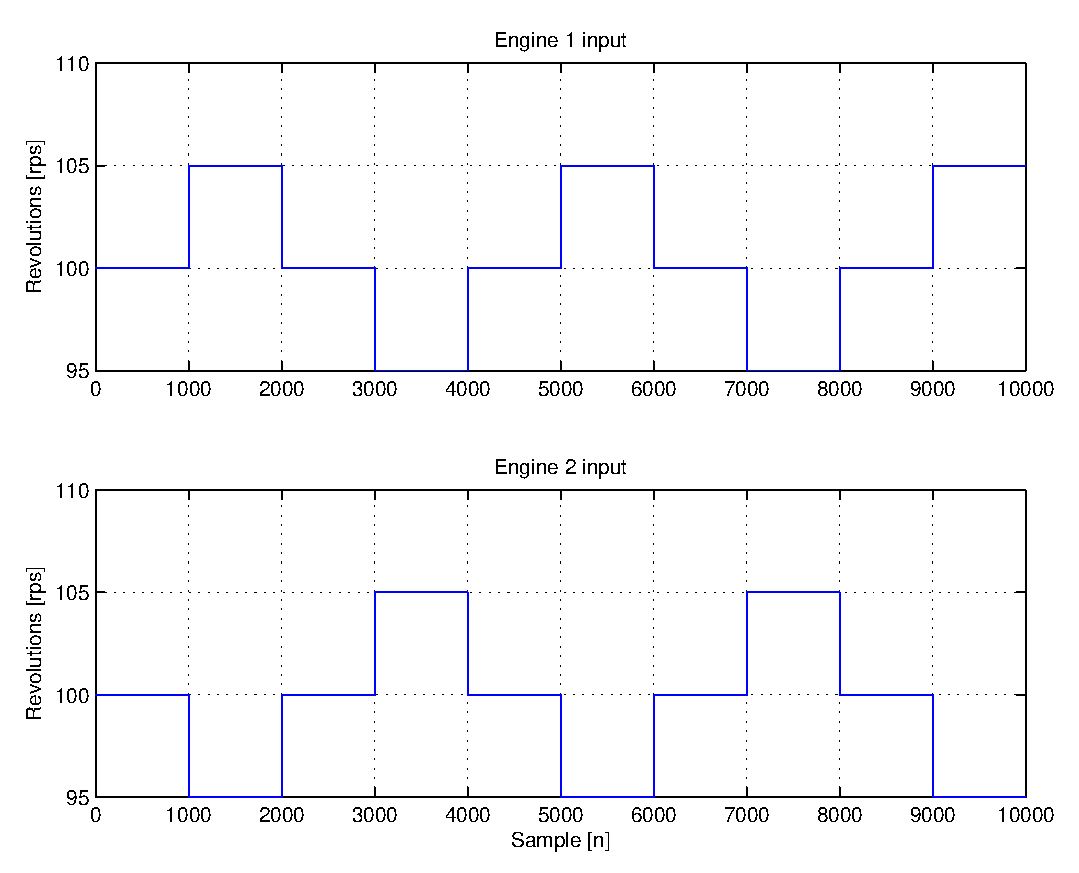
\includegraphics[width=\textwidth]{img/revol}
	\caption{Test input to the system}
	\label{fig:revol}
\end{figure}

As these cannot be measured accurately, we need to add noise to the input signals.

SETTING THE MEASUREMENT TO ZERO IF THERE IS NO SAMPLE to ensure that you still get a computation, without having a measurement - henvisning til Jespers første forelæsning!

Foreslag til Paper: Hvor langt ned kan man gå i sampling på GPS'en for at spare båndbredde, uden at miste præcision!

\subsection{Simulations of the filter}
% Text about linearizations / further computation.
Simulation of the Kalman filter have proven to provide an accurate estimate, however - the actual variances have to be measured. 

To avoid computational problems the Joseph Form of the Kalman Filter can be used. This ensures that the matrices used in the updating step is non-singular and positive definite. 

A little on the theory of Joseph Form.

\section{Position estimation}
During the development of the Kalman filter a lot or problems were discovered. One is to estimate the variances of the different measurement devies. The GPS delivers a position in latitude longitude format - which is converted into an x and y coordinate by rotating the entire system and shifting the local frame of the ship as a surface tangent to the earth. This will of course only be an estimate, but as the curvature of the earth is relatively small. The distance to the horizon can be estimated by $d \approx 3.57\sqrt{h}$ which on the ground, equals that the distance to the horizon is approximately 3.57 kilometers. As the areas to be measured are defined by a local bounding box - this area will to be defined to be smaller than 3.5 kilometers.

This section will contain the different things we've considered during the miniproject in Kalman filtering, and will be used to give a better estimate of the actual position (from the measurements implemented on the ship).

Below is a description of the measurable inputs to the system. These are obtained from a \ac{GPS} and a \ac{IMU} mounted on the ship.
Position and velocity from the \ac{GPS}: rotated coordinates (from LatLon to Local frame)
Linear acceleration from the \ac{IMU}: accelerometer
Angular acceleration from the \ac{IMU}: gyrometer
Angle from the \ac{IMU}: magnetometer (compass)

Estimating the bias of added wind and water current. As the wind and current shifts the ship around, and changes the torque to allow for a bias. This can be dealt with by extending the Kalman filter, to include these as measurements, and then subtracting these in the end result. This results in a filter that does not deal with the bias directly, but instead estimates without looking in to this. 

\begin{align}
\vec{A}_{ext} = \begin{bmatrix}
\vec{A}\\
\bar{\vec{b}}
\end{bmatrix}
\end{align}
\noindent Where:
\begin{ffk}
$\bar{\vec{b}}$ is the vector representing the bias in the x- and y-direction. 
\end{ffk}

\MATLAB plot indsættes af hvordan dette ser ud! (med og uden bias!).

The signal from the GPS can be seen as the actual position, plus some noise. 
